
\chapter{Multivariate Analysis and Machine Learning} \label{app:MVA}

In the broad class of problems known as classification, distinct features of events can be taken advantage of to label the event as a product of a signal process or background process. Over the last several decades, methods to approach this problem have grown increasingly sophisticated, using a multi-dimensional observable space rather than univariate techniques. These algorithms broadly are known as \glsfirst{MVA} algorithms.

%TODO: fill in the difference between ML and MVA

\gls{ML} can be separated into two broad categories: supervised and unsupervised learning. Supervised learning aims to learn a mapping from inputs to outputs, utilizing labeled data for training. Unsupervised learning works from unlabeled data in order to infer information and patterns about the dataset. The \gls{ML} methods used in this thesis all fall under the former label. Through the simulation methods (outlined in Section \ref{sec:simulation}), the physics process present in any given \gls{MC} sample are known, and this truth information is leveraged as the ``label'' of the data, making the problem suitable for a supervised classification task.

More specifically, the tasks presented in this thesis fall under the problem known as classification, where a model is trained to map inputs to outputs $y \in \{1,...,C\}$ for $C$ classes. Commonly $C=2$, known as binary classification, trying to isolate signal from background.  

The ``learning'' process in \gls{ML} is an updating of internal weights and biases in order to minimize of some \textit{loss function}. Table \ref{tab:loss-functions} lists loss functions typically used with various tasks commonly approached by \gls{ML} methods (this list is certainly not exhaustive).

\begin{table}[!ht]
    \centering
    \begin{tabular}{c|c}
        Task                  & Common Loss Function \\
        \cline{1-2}
        Binary Classification     & Binary Cross-Entropy\\
        Multiclass Classification & Categorical Cross-Entropy\\
        Regression                & Mean Squared Error
    \end{tabular}  
    \caption[A list of common tasks in which \gls{ML} is employed, and loss functions typically used.]{A list of common tasks in which \gls{ML} is employed, and loss functions typically minimized in setting biases and weights for \gls{ML} models.}
    \label{tab:loss-functions}
\end{table}


\section{General Principles and Terminology}

This section will overview some general concepts relevant to \gls{ML} methods and referenced within this thesis.

\noindent\textbf{Hyperparameters}\\
\indent When developing \gls{ML} algorithms, tuning is generally done by manipulating the ``hyperparameters'' of the algorithm. These are properties that define the parameters of the algorithm itself - its topology, how it learns, etc. Hyperparameters are fixed before the learning process begins. For most hyperparameters, there is no a priori assumption of the best values, and optimization through successive model trainings with differing values is required.

\noindent\textbf{Training and Testing Sets}\\
\indent A major concern when developing a fitting model is known as \textit{overfitting}, in which a model is overconstrained to model the particular data it is trained on, and thus not generalizable and not useful for inference. To avoid overfitting, before training data is often split into subsamples. The training sample is used to fit the model, setting the weights and biases. Once fit, the model is applied to the testing set to evaluate performance\footnote{In some cases, a third set of data known as a ``validation'' set is used. In this case, the training data is used for initial fitting and the validation set is used for hyperparameter optimization.}. Significant differences in performance between the training and testing sample is an indication of overfitting, while a similar performance suggests a model is generalizable to new data.



\section{Algorithms}

In the work presented in this thesis, two primary machine learning algorithms are used: Boosted Decision Trees and Neural Networks. The following sections will outline those methods.

\subsection{Rectangular Cuts}

Although not \gls{ML}, one classical univariate method for signal selection is known as rectangular cuts. In this, a feature of the data set is cut at a single point, and values either above or below that are taken as the signal. Performing this procedure along many different input variables yields a signal region that mathematically appears like a N-dimensional hypercube, where N is the number of variables cut upon. 

Optimization of a rectangular cuts method usually involves calculating a \gls{FOM} (such as categorical accuracy or Asimov significance) at each possible cut along the N-dimensional space. As a result, cut selection can be dependent on the granularity of the scan and to reduce overconstraining cuts to be dataset dependent, segmenting into training and testing samples is good practice for optimization.

\subsection{Boosted Decision Tree}

The fundamental idea of a decision tree is a familiar one. Input data is split based on discriminating features, each level of the tree creating a new split (called node) motivated by best separating data from the target class from background data. This procedure is repeated until a stopping condition is met, typically either minimum number of samples in a node or a maximum tree depth is achieved (both hyperparameters). Once final splits have been made, the predominant sample type present in a node is assigned to all of the data in that node. A pictorial diagram of this logic can be found in figure \ref{fig:bdt}.

\begin{figure}[!ht] 
    \centering
    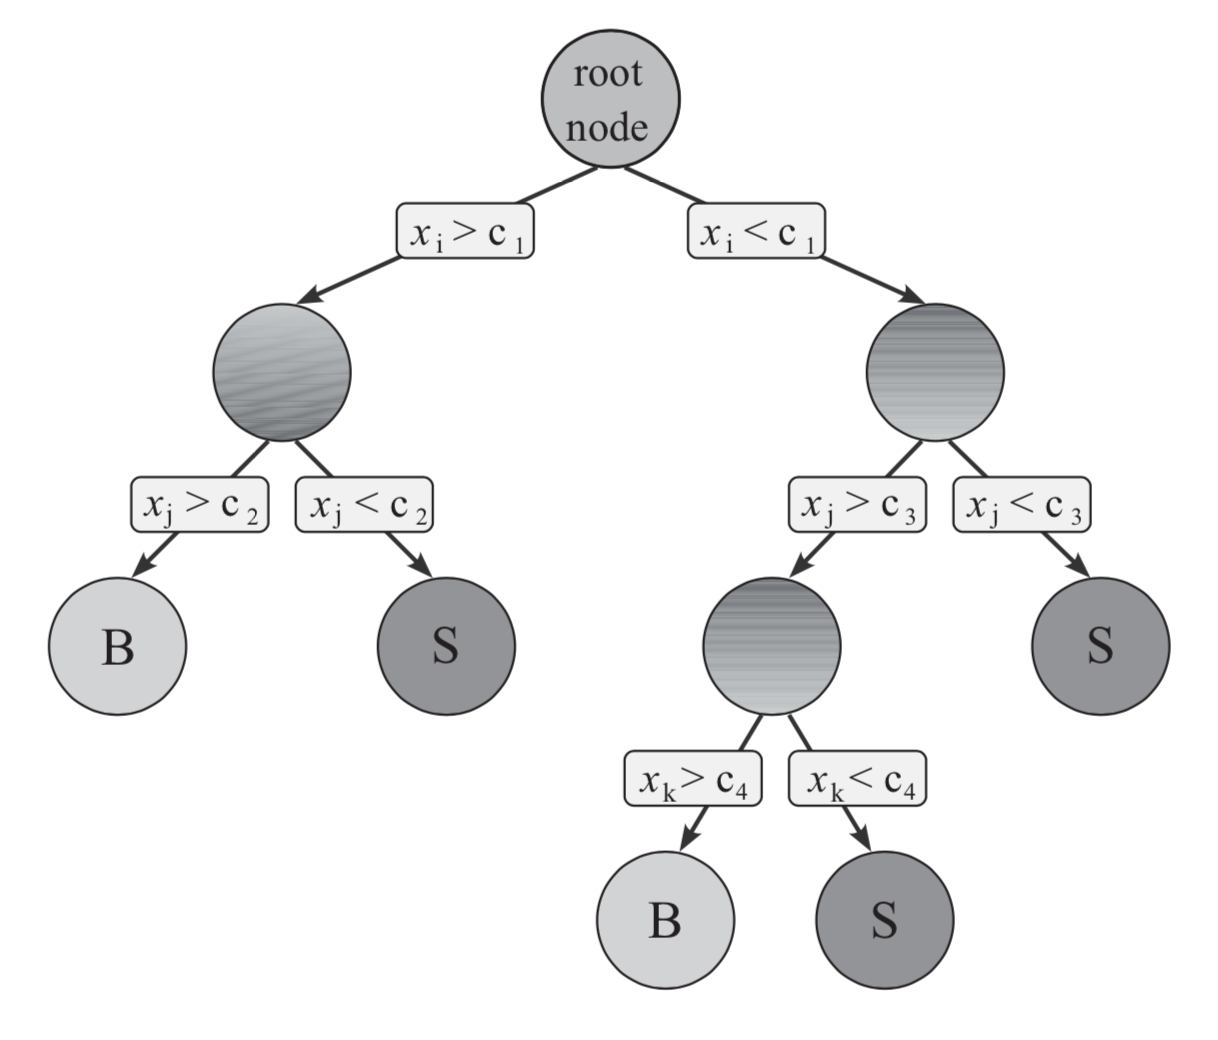
\includegraphics[width=.7\textwidth]{appendices/images/bdt.png}
    \caption[A diagram of a single decision tree]{A diagram of a single decision tree, where data is split on properties $x_N$. The presented tree has a maximum depth of 3, and is classified into either signal (S) or background (B) in stopping nodes \cite{data-analysis}.}
    \label{fig:bdt}
\end{figure}

Single decision trees do not typically do a good job at classification tasks, so the principle of ``boosting'' is used in order to improve the classification accuracy. Boosting is a type of ensemble method, which are a class of methods that combine the output of many weak learners (classifier with small correlation to truth) to form one strong learner (classifier well-correlated to truth). In boosting, single decision trees are trained, then misclassifications within that tree are identified and up-weighted in the next iteration. All of the trees are ultimately combined to create the final strong learner, called a \glsfirst{BDT}. 

Via this construction, cutting on a \gls{BDT} score gives a more flexible solution space than that of a rectangular cuts method.

There are various different boosting methods, notably ``Adaboost'' \cite{adaboost} and ``Gradient Boosting'' \cite{gradBoost}, which generally differ by the definition of their loss function.


\subsection{Neural Networks}

An Artificial \glsfirst{NN}\footnote{Historically, these have been abbreviated ANN for ``Artifical Neural Network,'' however to avoid ambiguity with modern ``Adversarial Neural Networks,'' the abbreviation NN is used.} is a nonlinear machine learning algorithm that attempts to perform a task via a combination of nonlinear basis functions ($h(x)$) where weights ($w$) are learned in the training procedure\footnote{The name ``Neural Network'' comes from such models being inspired by neurological structures. At each neuron, signals are received by dendrites, passed along an axon to produce some output, which is passed along through axon terminals. Many of these neurons come together to process sophisticated information. This loosely mirrors the topology of an \gls{NN}, where basis functions parallel neurons.}. The resulting function is:

\begin{equation}
    y(x) = w_0^2 + \sum_{m=1}^{M} \big [w_m^2 \cdot h \big (w_{0m}^1 + \sum_{k=1}^{D} w_{km}^1 x_k) ]
\end{equation}

Where $D$ is the number of inputs and $M$ is the number of basis functions. Here $h$ is known as an \textit{activation function}, and given a summation over enough of these activation functions, any possible function can be approximated \cite{nn-basis}. Common choices are:
\begin{itemize}
    \item The sigmoid function, given by $h(t) = 1/(1+e^{-t})$.
    \item The hyperbolic tangent function, given by $h(t) = (e^t - e^{-t}/(e^t + e^{-t}))$.
    \item The rectified linear unit (ReLU), given by $h(t)=max(0,x)$, in other words, returning 0 below $x=0$ and $y=x$ otherwise.
\end{itemize}

An illustration of a \gls{NN} with $D=4$ and $M=5$ is shown in Figure \ref{fig:nn}. 

\begin{figure}[!ht] 
    \centering
    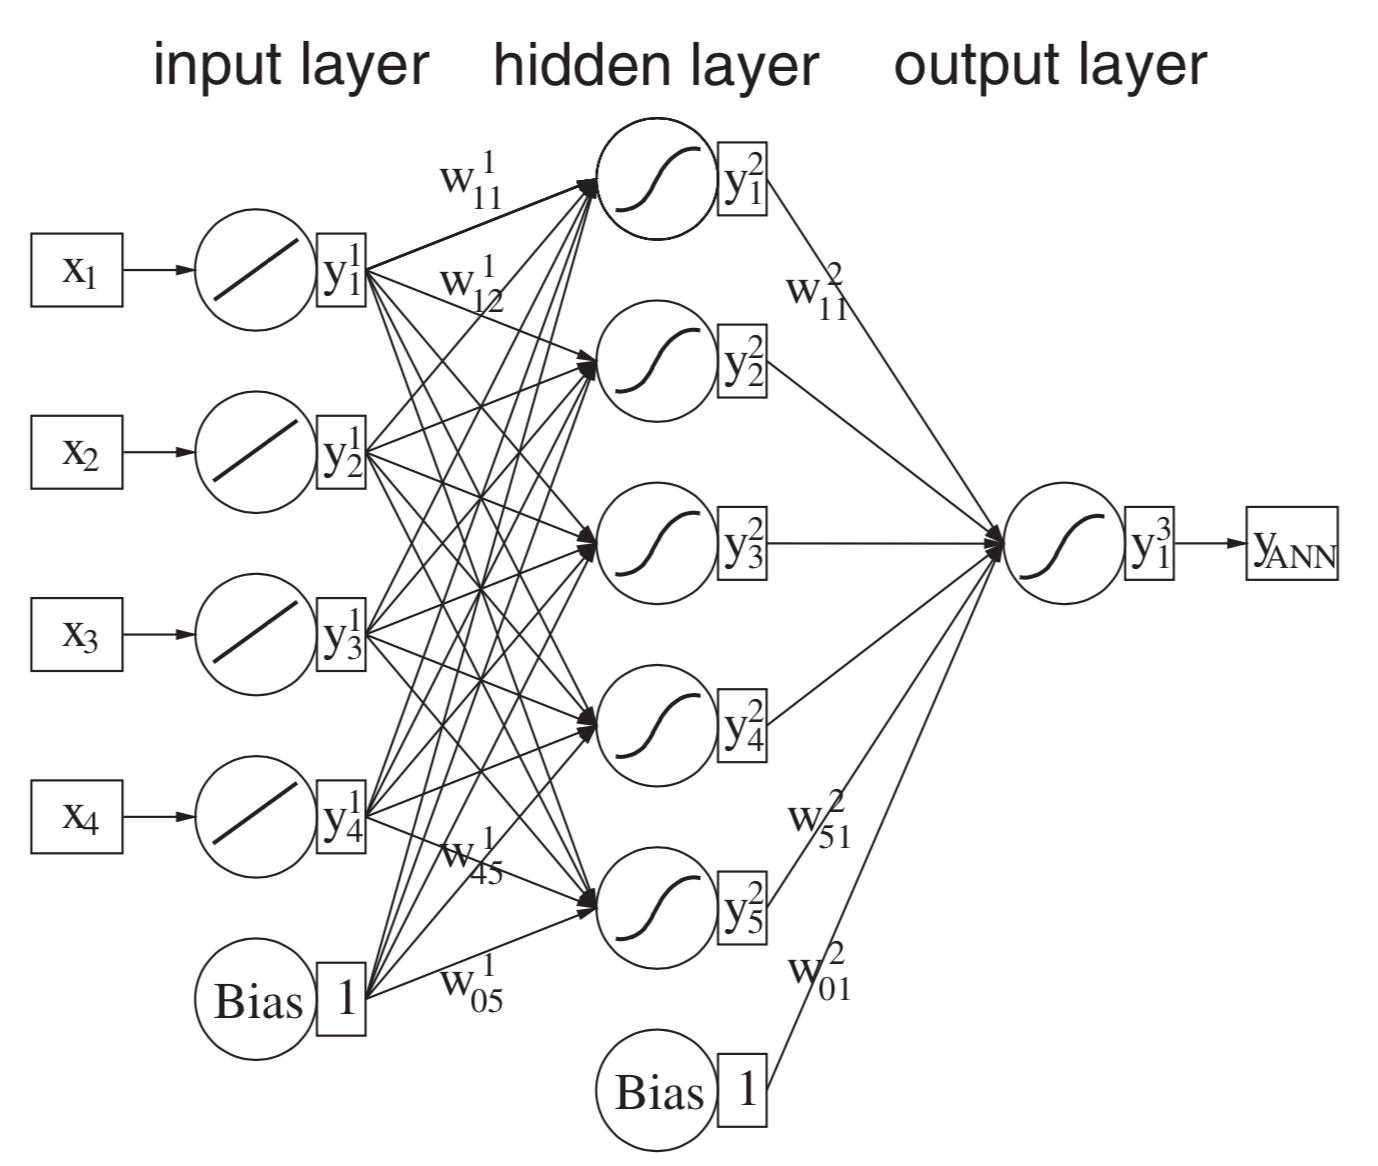
\includegraphics[width=.7\textwidth]{appendices/images/neural_network.png}
    \caption[A sample \gls{NN} with $D=4$ and $M=5$]{A sample \gls{NN} with $D=4$ and $M=5$ \cite{data-analysis}.}
    \label{fig:nn}
\end{figure}

